\chapter{システムの設計・実装}
\label{chap:implementation}

\section{UoIP} % UHD over IP

\section{システム構成}

\section{ソフトウェアによる実装}

\section{ハードウェアによる実装}

\subsection{FPGAの回路設計}

Axi4-Stream、tuser
図\ref{fig:fpga-video-ethernet-diagram}
図\ref{fig:fpga-ethernet-video-diagram}

本実装では、Xilinxの 10 Gigabit Ethernet Subsystem、及び、Video Processing Subsystemを用いる。
10 Gigabit Ethernet Subsystemの挙動に空いては、Xilinx PG157\cite{xilinx-pg157}を参照されたし。
\cite{xilinx-pg235}
\cite{xilinx-pg236}

\begin{figure}[htbp]
    \begin{center}
        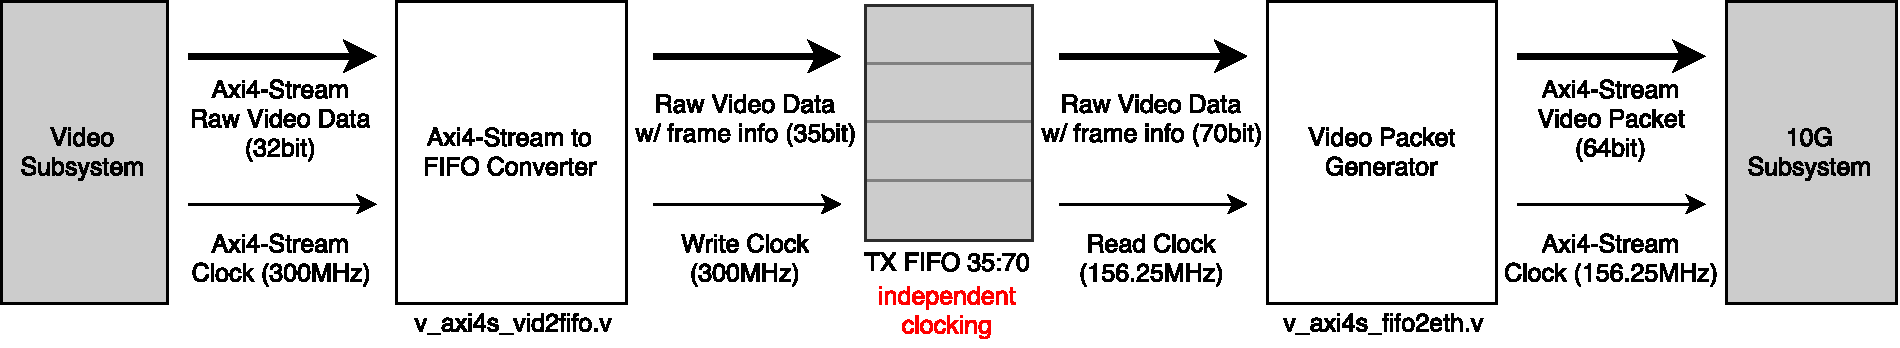
\includegraphics[bb=0 0 911 166,width=15.5cm]{img/fpga-video-ethernet-diagram.pdf}
    \end{center}
    \caption{Video Stream to Ethernet Packet Subsystem Diagram}
    \label{fig:fpga-video-ethernet-diagram}
\end{figure}

\begin{figure}[htbp]
    \begin{center}
        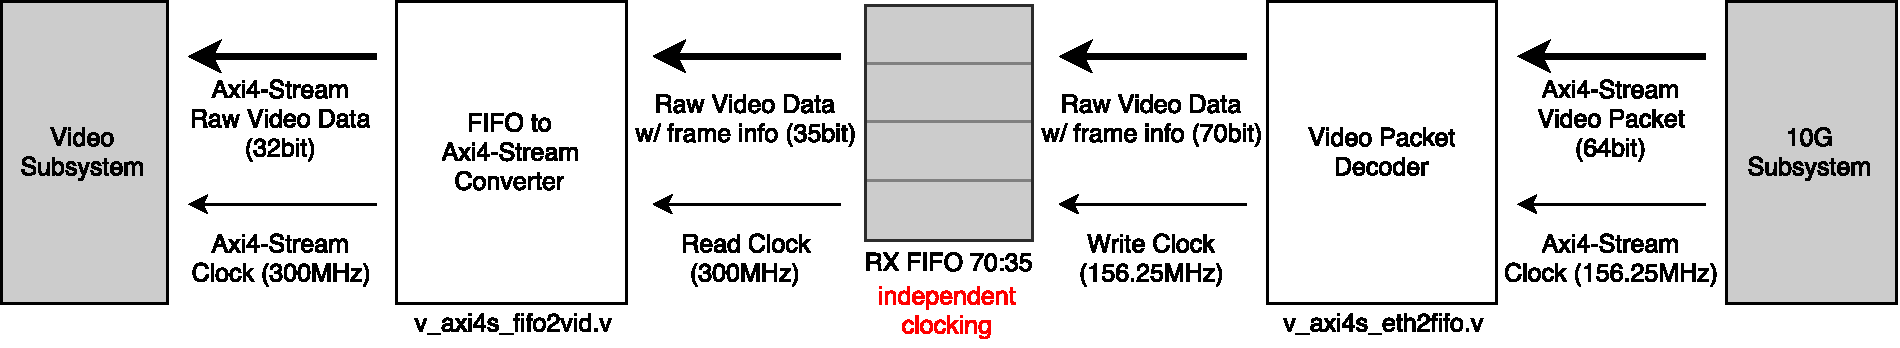
\includegraphics[bb=0 0 911 166,width=15.5cm]{img/fpga-ethernet-video-diagram.pdf}
    \end{center}
    \caption{Ethernet Packet to Video Stream Subsystem Diagram}
    \label{fig:fpga-ethernet-video-diagram}
\end{figure}

図\ref{fig:fpga-video-packet}に、本実装で用いたパケット構造を示す。

\begin{figure}[htbp]
    \begin{center}
        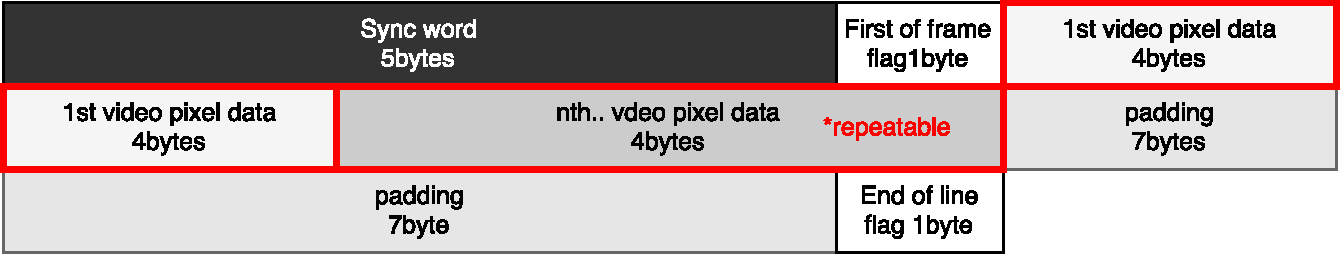
\includegraphics[bb=0 0 641 161,width=15.5cm]{img/fpga-video-packet.pdf}
    \end{center}
    \caption{Video Packet Structure}
    \label{fig:fpga-video-packet}
\end{figure}
